\section{Un poco de historia....}

\begin{wrapfigure}{r}{0.35\textwidth} \centering
  \includegraphics[keepaspectratio,width=0.3\textwidth]{Imagenes/06.02.vor.imagenes/Marconi.eps}\caption{Guillermo Marconi}
\end{wrapfigure}


Las radioayudas utilizadas actualmente (VOR, DME, ILS, etc.) se remontan a los primeros d\'ias de la radiocomunicaci\'on. Sus l\'ineas de origen se cruzan en muchos puntos, pero  encuentran, finalmente, su inicio en dos patentes registradas en Alemania en 1906.

Hacia 1905 Marconi hab\'ia dedicado un esfuerzo considerable a la investigaci\'on de las propiedades de la cl\'asica antena en L invertida. Encontr\'o que si el tramo horizontal era considerablemente mayor que el vertical, el diagrama polar presentaba un abombamiento considerable en la direcci\'on contraria a la l\'inea de secci\'on horizontal.

En 1905 patent\'o un sistema que utilizaba este tipo de antenas tanto para la emisi\'on como la recepci\'on, reivindicando excepcionales propiedades direccionales para la combinaci\'on. Bas\'andose en el mismo principio, Marconi registr\'o al a\~no siguiente la patente de un sistema con un n\'umero de antenas L invertidas igualmente espaciadas en forma radial alrededor del receptor. Seleccionando la antena que recib\'ia la se\~nal m\'as intensa pod\'ia averiguarse la direcci\'on aproximada de la estaci\'on emisora.

\begin{wrapfigure}{l}{0.35\textwidth}
  \centering  \includegraphics[keepaspectratio,width=\linewidth]{Imagenes/06.02.vor.imagenes/Telefunken.eps}
    \caption{La "br\'ujula"\, Telefunken} \label{fig:brujula.telefunken}
\end{wrapfigure}


Antes de que pasara un a\~no, Telefunken, en Alemania, hab\'ia introducido una idea muy parecida pero utilizando la parte emisora. Consist\'ia en un emisor que radiaba primero una se\~nal de inicio preestablecida a una antena central omnidireccional, seguida de una segunda emisi\'on en cada una de las 32 antenas espaciadas radialmente alrededor del radiador central omnidireccional y situadas seg\'un las marcaciones de la br\'ujula (Figura \ref{fig:brujula.telefunken}).

Una estaci\'on que desease utilizar la baliza, s\'olo ten\'ia que accionar un cron\'ometro al o\'ir la se\~nal de inicio y detenerlo cuando la se\~nal alcanzaba su m\'axima intensidad. Como ayuda a los usuarios del sistema se dise\~no un reloj especial. Ten\'ia una aguja que completaba una revoluci\'on en 32 segundos y su esfera estaba calibrada seg\'un los puntos de la br\'ujula.

Aunque este sistema no alcanz\'o nunca un uso generalizado, se le puede considerar como el precursor de todos los radiofaros giratorios modernos.

\begin{wrapfigure}{r}{0.35\textwidth} \centering
  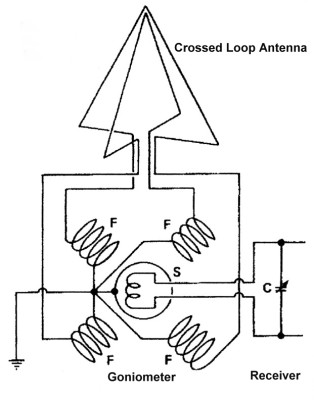
\includegraphics[keepaspectratio,width=\linewidth]{Imagenes/06.02.vor.imagenes/bellinitosiprinciple.jpg}\caption{Principio del equipo de Bellini y Tosi}
\label{fig:bellini.y.tosi.principio}
\end{wrapfigure}

En 1907 Bellini y Tosi presentaron un dise\~no que comprend\'ia dos antenas receptoras de cuadro cruzadas a 90 grados a partir de las cuales se pod\'ia determinar la direcci\'on de las ondas incidentes, mediante la magnitud relativa de las corrientes que se induc\'ian en las antenas (Figura \ref{fig:bellini.y.tosi.principio}). Este sistema alcanz\'o un desarrollo ulterior y, durante la Primera Guerra Mundial (1914-1948), ambos contendientes depositaron una confianza considerable en el mismo. Pese a que una estaci\'on radiogonom\'etrica s\'olo pod\'ia controlar a un avi\'on a la vez y que, a veces, debido a desconocidos fen\'omenos de propagaci\'on, surg\'ian errores posicionales de mas de 50 millas; Von Buttlar-Brandenfels, el \'unico comandante de Zeppelin que vol\'o durante toda la guerra dedujo que la radionavegaci\'on era muy superior a la navegaci\'on astron\'omica.

\begin{figure}[!hbt]
  \centering  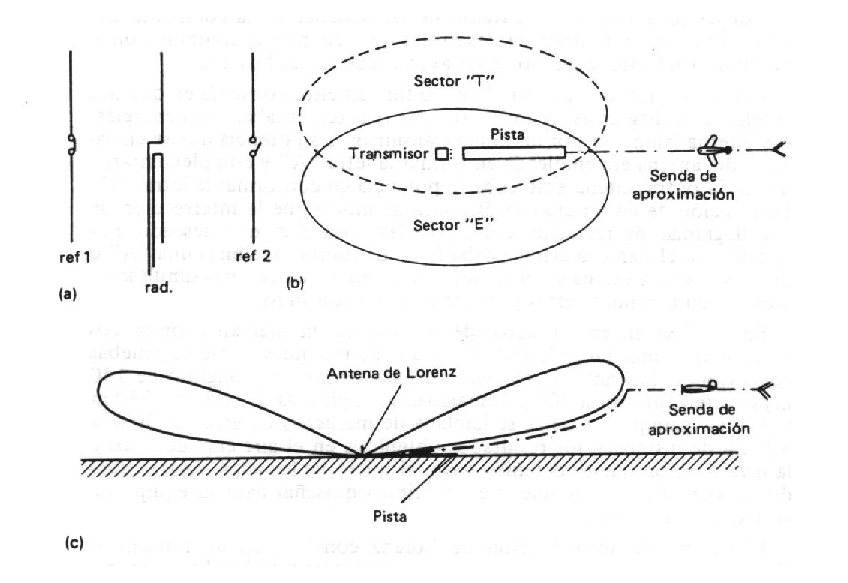
\includegraphics[keepaspectratio,width=0.8\textwidth]{Imagenes/06.02.vor.imagenes/Loran.eps}
    \caption{El sistema de aproximaci\'on de Lorenz.
	(a) Dispositivo de antenas. (b) Modelo de radiaci\'on. (c) Diagrama polar vertical y senda de aproximaci\'on.
}
    \label{fig:sistema.lorenz}
\end{figure}

A partir de 1916, Marconi inici\'o el estudio de radioenlaces direccionales de onda corta en una serie de experimentos que fueron llevados a cabo con diversas alternativas en Hendon y Cernavon, a partir de los cuales se desarroll\'o el ``\emph{faro de radioenlaces}'' que fue instalado en 1921 en Inchkeith Island. El hecho m\'as importante en el dise\~no de este equipo fue que \'unicamente pod\'ia generarse un haz suficientemente localizado como para proporcionar una exactitud digna de consideraci\'on, elevando la frecuencia al espectro de VHF. Adem\'as, el dise\~no de los sistemas de manipulaci\'on no permit\'ia que la baliza radiase informaci\'on err\'onea; asimismo el empleo del cron\'ometro se hizo innecesario.

Volviendo a 1907, una patente de O. Scheller de la compa\~n\'ia Lorenz, condujo a una l\'inea de desarrollo que, cuando se combin\'o con el radiofaro rotatorio de Marconi, culmin\'o con las radioayudas de hoy en d\'ia.

Era el ``Indicador de rumbo'', cuyo fundamento consist\'ia en que dos antenas con diagramas de radiaci\'on que se interceptaban, eran energizadas alternativamente por un \'unico transmisor. La potencia que se enviaba a una antena era utilizada para formar la letra ``A'' y la otra antena formaba la ``N''. La posici\'on de las antenas se dispon\'ia de tal manera que la intersecci\'on de sus diagramas de radiaci\'on correspondiese con el rumbo deseado. Por lo tanto, si una aeronave se encontrase fuera de rumbo, recibir\'ia una ``A'' o una  ``N'', pero si se encontrase en el rumbo, oir\'ia ambas simult\'aneamente, combin\'andose estas para dar un tono continuo.

En 1917 se realizaron experiencias en Alemania con barcos y cinco a\~nos m\'as tarde, Keibitz las realiz\'o con aviones. Aunque en tierra se hablaba de un margen de error de 30 m a 3,5 km de distancia, los resultados obtenidos fueron dudosos y la investigaci\'on qued\'o detenida hasta comienzos de la d\'ecada de 1930 cuando la compa\~n\'ia us\'o de nuevo el principio equise\~nal para su equipo de aproximaci\'on de VHF.

Este equipo de aproximaci\'on de Lorenz consist\'ia en un transmisor de VHF situado en la cabecera de la pista de aterrizaje y trabajaba a una frecuencia de aproximadamente 33 Mhz. Este sistema alimentaba un dipolo vertical a cuyos lados, formando \'angulo recto con la pista, se situaba un elemento reflector. El punto medio de cada uno de estos elementos reflectores estaba interrumpido y puenteado por
\begin{wrapfigure}{l}{0.45\textwidth} \centering
  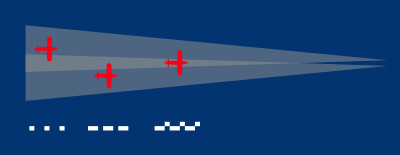
\includegraphics[width=\linewidth]{Imagenes/06.02.vor.imagenes/Lorenz_beam.png}
%  \caption{\centering Se\~nales de Lorenz  \\{\tiny fuente: \url{http://en.wikipedia.org/wiki/Lorenz_beam }}} \label{fig:seniales.lorenz}
\end{wrapfigure}
un conjunto de contactos de rel\'e que operaban en oposici\'on, esto es, si un conjunto de contactos se encontraba cerrado el otro estar\'ia abierto, manteniendo sin funcionar ese reflector. Operando sobre los rel\'es, el diagrama de radiaci\'on pod\'ia ser trasladado de uno a otro lado. Ambos diagramas se interseccionaban sobre la l\'inea central de la pista  (Figura \ref{fig:sistema.lorenz}). La manipulaci\'on de los receptores se hac\'ia de modo que uno de ellos se manten\'ia en funcionamiento un per\'iodo de tiempo tres veces mayor que el otro; as\'i, cuando un piloto se aproximaba a la pista ligeramente fuera de rumbo, escuchaba una serie de ``E'' ($\cdot \, \cdot \, \cdot$) o de ``T'' ($- \, - \, -$) que se fund\'ian en un tono continuo ($- \cdot - \cdot - \cdot$) si se encontraba en el rumbo adecuado (Figura \ref{fig:seniales.lorenz}). Este sistema se denomin\'o \emph{Ultrakurzwellen-Landefunkfeuer} (LFF), o radiobaliza de ondas ultra-cortas para aterrizaje.


El receptor del avi\'on estaba dotado de un medidor de intensidad de se\~nal y pod\'ia obtenerse una gu\'ia de la senda de planeo siguiendo un contorno de igual intensidad de campo.

Este sistema se tambi\'en en Inglaterra con \'exito y se mantuvo en servicio hasta principios de 1960.

% \begin{figure}[!h]
%   \centering
%   \subfigure[Torre de control aeropuerto de Croydon (Inglaterra) coronada por los cuadros radiogonom\'etricos Bellini-Tosi {\tiny Fuente: \url{http://www.thecinetourist.net/the-hotel-bristol-enigma.html}}]{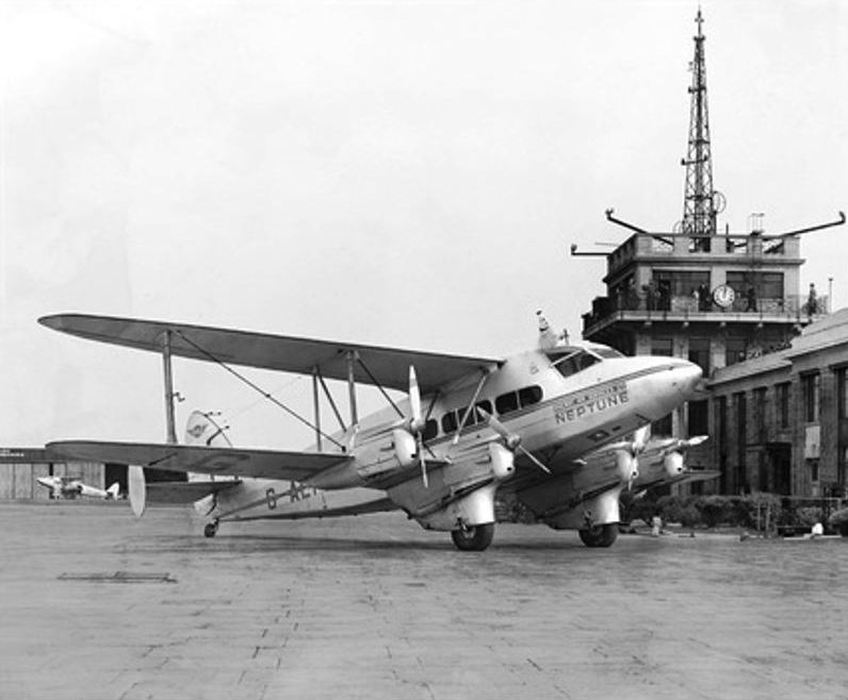
\includegraphics[height=6.0cm]{Imagenes/historia/croydon-control-tower-02.jpg}} 
%   \subfigure[Receptor radiogonom\'etrico Bellini-Tosi \\{\tiny Fuente: \url{http://www.airwaysmuseum.com/B-T\%20MFDF\%201.htm}}]{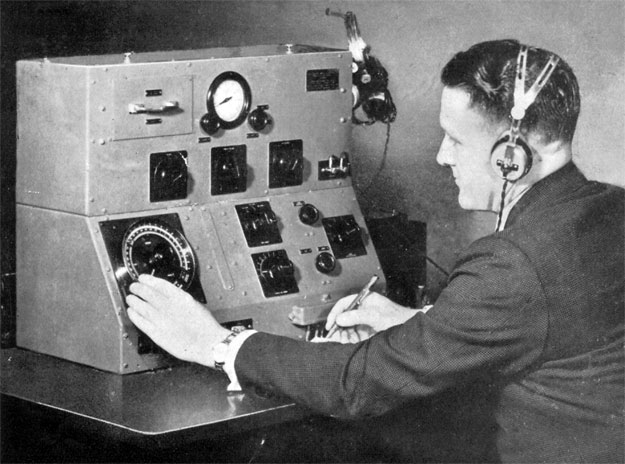
\includegraphics[height=6.0cm]{Imagenes/historia/bellini-tosi-medium-frecuency-direction-finder.jpg}}

%   \caption{Equipo de tierra sistema radiogoni\'ometro}
%   \label{fig:radiogoniometro}
% \end{figure}

En Estados Unidos se investig\'o, por la misma \'epoca, un sistema de antenas ortogonales mediante se\~nales enclavadas. Este m\'etodo generaba cuatro rumbos independientes por cada estaci\'on y se le atribu\'ia una buena apreciaci\'on. 

Desde 1923 a 1926 se continu\'o esta l\'inea, descubri\'endose que utilizando un goni\'ometro transmisor junto con cuadros Bellini-Tosi, los rumbos pod\'ian ser desplazados casi a cualquier direcci\'on deseada. El \'exito del sistema fue tal que a comienzos de 1926 se emprendi\'o la labor de instalar un sistema de estas radiobalizas para trazar el creciente n\'umero de l\'ineas a\'ereas dentro de ese pa\'is. 

Posteriormente se encontr\'o que el sistema de antenas Bellini-Tosi presentaba errores de m\'as de 40 grados en condiciones nocturnas desfavorables, pero su sustituci\'on por antenas Adcock resolvi\'o este problema. En 1944 exist\'ian m\'as de 300 de estos equipos que permanecieron en servicio hasta ser reemplazados por el VOR.


Debido a los problemas inherentes al manejo de radiofaros omnidireccionales de frecuencias medias (efectos nocturnos, etc) en 1937 la U.S. Civil Aeronautics Administration llevó a cabo una serie de pruebas con el uso de VHF para radiofaros omnidireccionales. Las primer las pruebas usaban una frecuencia de 63 MHz y los resultados fueron prometedores, pero surgieron problemas debidos a efectos de reflexión bajo condiciones de propagaci\'on anormales y, en consecuencia, la frecuencia fue elevada a 12S MHz. Aunque todavía subsistían algunos problemas con los sistemas de cuatro rumbos, el trabaJo con VHF había demostrado que el equipo que trabajaba con estas frecuencias era capaz de obtener mejores resultados que el de MF. De todos modos, un problema importante que quedaba por resolver era la desorientación que experimentaba un piloto cuando perdía sus marcaciones cerca de un radiofaro de cuatro rumbos ; por eso se investigȯ la viabilidad de un sistema de radiofaro de dos rumbos, en el cual se emitian a la vez dos modelos de radiación que conformaban cuatro rumbos distintos. Típicamente podía consistir en un rumbo este-oeste definido por señales de 150 Hz y otro norte-sur de 90 Hz, separándose estas señales mediante filtros en el receptor del avión para alimentar diferencialmente un medidor con el cero en posición central. Esto se conoció como rumbo visual. Adicionalmente se instrumentaron un par de rumbos norte-sur en ángulo recto usando senales interconexionadas del tipo de Lorenz.% (D y U)

Hacia 1936 tambi\'en se consideró un radiofaro que radiaba un n\'umero infinito de rumbos, que era esencialmente un retorno al radiofaro giratorio.

Dicho radiofaro empleaba un sistema en el que el diagrama polar horinzontal tenía forma de cardioide, con la propiedad de que al girar, la intensidad de la señal en cualquier estación receptora variaba sinusoidalmente. El diagrama giraba a 60 Hz. La onda sinusoidal recibida era separada en dos partes en cuadratura de fase, que eran conectadas a las placas
de deflexión de un tubo de rayos catódicos. Esto producia una traza
circular, cada punto de la cual estaba asociado con el instante correspondiente a 
alguna orientaci\'on particular del diagrama espacial, pero sin
ningún punto de referencia. Este fue suministrado al principio introduciendo una discontinuidad en la se\~nal cuando el m\'aximo del diagrama
giratorio pasaba por el norte verdadero, siendo el resultado una deflexi\'on radial en la traza que,
 de otro modo, sería circular, proporcionando así una indicación del rumbo. 

En los primeros trabajos sobre dicho radiofaro se usaba una frecuencîa de 6,5 MHz, 
pero en vista de la tendencia en favor del uso de VHF
cesaron las pruebas con esta frecuencia y posteriormente se usaron frecuencias en la banda de 125 MHz.

Una versi\'on pasterior del equipo sustituía la discontinuidad instantánea de referencia
 por una modulaci\'on a 60 Hz de una subportadora de 1O kHz cuya fase se hacía coincidir con el diagrama
 giratorio en el norte verdadero.

En el receptor se comparaban las fases de la se\~na1 de referencia y de
la se\~nal g\'irada, correspondiendo la diferencia de fase con el rumbo
del receptor. Debido a esta modificaci\'on en la se\~nal de referencia 
se dej\'o de usar como \'indicador el tubo de rayos catódicos, 
que fue sustituido
por un medidor de fase con \'indicac\'i\'on azimutal.

Esto era, en esencia, el VOR que se usa hoy día, consist\'iendo las
principales variaciones posteriores en un cambio en la frecuencia para
usar la banda de 112,0 MHz a 117,9 MHz, en una reducción de la velocidad 
de rotaci\'on del d\'iagrama girator\'io y en una modulación de referenc\'ia
 de 30 Hz usando 9960 Hz para la frecuencia subportadora.


% Durante la Segunda Guerra Mundial se produjeron avances notables para el guiado y la navegaci\'on a ciegas de las aeronaves, con el fin de realizar bombardeos de precisi\'on. 

% Los alemanes utilizaron el principio del sistema de aproximación Lorenz para sus raids de bombardeo a ciegas, principalmente el 
% Knickebein ('Pierna torcida') y el X-Ger\"{a}t ('Aparato-X'),
% durante la ofensiva de bombardeo sobre las ciudades de Inglaterra en el 
% invierno de 1940/41.

% El X-Ger\"{a}t era muy similar al LFF de Lorenz, siendo mucho m\'as direccional y con mayores alcances. Usando las mismas frecuencias permit\'ia a los aviones utilizar los emisores LFF ya instalados, pero se necesitaba un segundo emisor para ubicar una localizaci\'on.

% Estos sistemas utilizaban haces cruzados de radiondas de las mismas caracter\'isticas pero de diferentes frecuencias, lo que permit\'ia al piloto calcular su velocidad, desde el momento en que cruzaba la se\~nal 
%  crossing the Fore Cross Signal and crossing the Main Cross Signal), and indicate when he should drop his payload. 
% Los c\'alculos se efectuaban mediante una computadora mec\'anica.

% Posteriormente Lorenz modific\'o este sistema creando el sistema de guiado lateral 
% Viktoria/Hawaii 
% para el misil V-2.
